\documentclass[12pt]{article}
\usepackage{amsmath}
\usepackage{fancyhdr}
\usepackage{hyperref}
\usepackage{graphicx}
\newcommand{\compactlist}{\setlength{\itemsep}{0pt} \setlength{\parskip}{0pt} \setlength{\leftskip}{-1em}}
\usepackage[top=0.9in, bottom=0.8in, left=0.9in, right=0.9in]{geometry}

\lhead{MATH 4263/5373}
\rhead{Nov. 5, 2019}
\chead[RE]{Comparison of interpolation and approximation}
\cfoot{}
%\rfoot{Code for figure and report is available in the class folder.}
\pagestyle{fancy}
\begin{document}
Given the data in the vehicle speed problems (see sections 3.3, 3.4 homework), we can plot a few functions representing the position data (see Figure~\ref{fig::plots}).  The Hermite (black) and spline (red) interpolations exactly pass through the position data points.  On the other hand, the linear approximation (blue) does not exactly pass through a single of these points.
%
\begin{figure}[h!]\centering
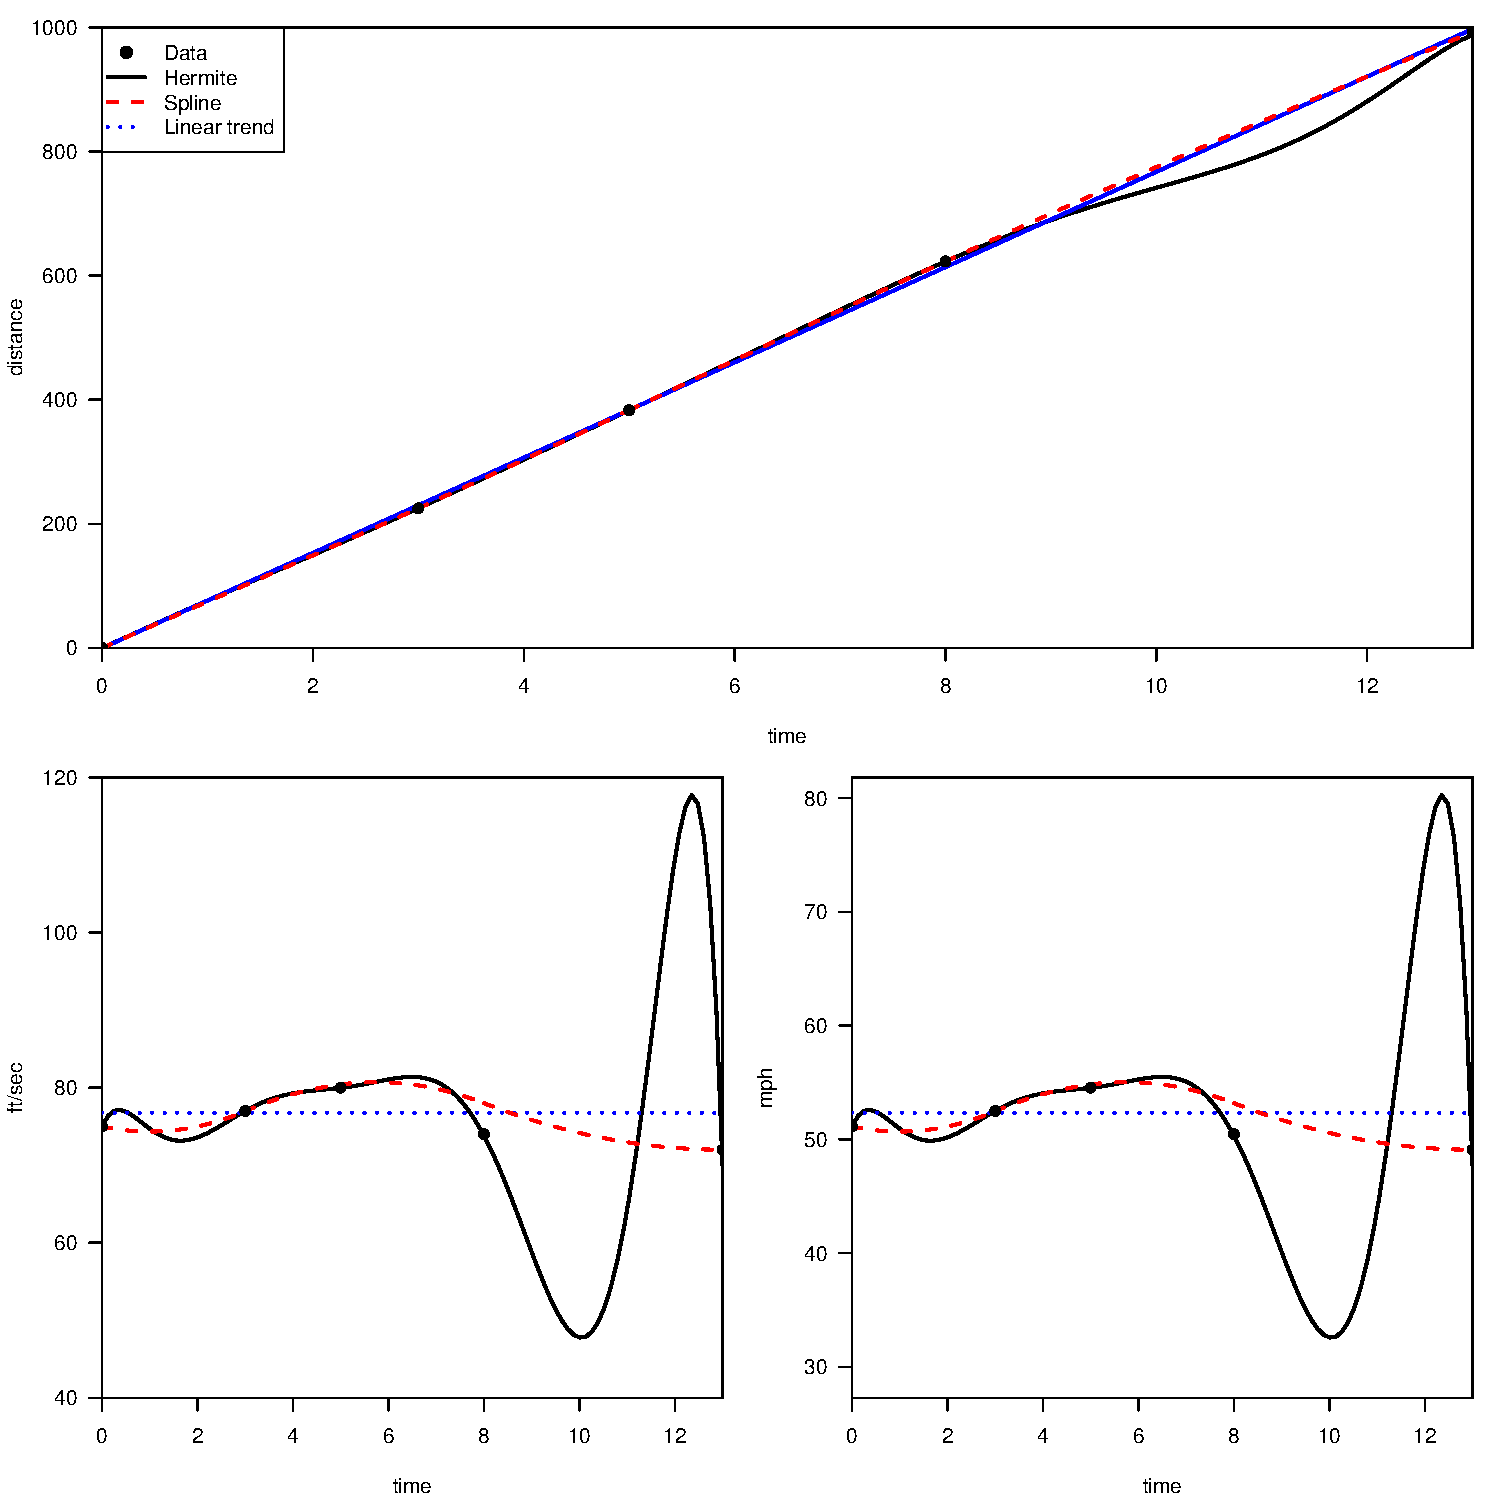
\includegraphics[width=\textwidth]{speed}
\caption{\textbf{Top:} Data and interpolating and approximating polynomials. \textbf{Bottom:} Speed data and predicted speed by interpolating and approximating polynomials (\textbf{left:} feet per second and~\textbf{right:} miles per hour).}\label{fig::plots}
\end{figure}

\noindent There are a variety of factors to weigh when choosing a method for representing data by a function.
%
%\begin{table}[h!]\centering
%\begin{tabular}{cc}
%\hline
%\(r\) & Sample shape or example\\
%\hline\hline
%\(0<r<1\) & square root function (\(r=0.5\))\\
%\(r=1\) & linear function \\
%\(r>1\) & quadratic or cubic functions
%\end{tabular}
%\end{table}

\end{document}